\chapter{METODOLOGÍA DE LA INVESTIGACIÓN}
\section{Diseño de la investigación}
En esta sección del documento se explicará cual es el diseño, el tipo y el enfoque del trabajo de
investigación, así como también la población y la muestra. 
%Para finalizar se explicará el
%proceso de aplicación de las redes neuronales convolucionales.
\subsection{Enfoque de la investigación}
El presente trabajo tendrá un enfoque cuantitativo ya que se busca diseñar y desarrollar instrumentos, en este caso modelos predictivos, para responder al problema estudiado a partir de medición de datos históricos en la plataforma Kickstarter con herramientas basadas en la estadística y matemáticas que puedan ser interpretadas por cualquier investigador. 

\subsection{Alcance de la investigación}
El alcance del presente trabajo será descriptivo ya que se recolectarán datos en un determinado rango de tiempo (desde 2009 hasta el presente año 2019) para describir el comportamiento de las campañas de proyectos tecnológicos en Kickstarter a partir de las características de sus variables y con ello, pronosticar su posible éxito o fracaso antes de finalizar la campaña con un nivel óptimo de precisión.

\subsection{Tipo de la investigación}
Para determinar el tipo de la investigación, primero es necesario definir el actual trabajo como Diseño Experimental ya que las variables que se tienen serán controladas, es decir, serán agregadas o quitadas en el o los modelos construidos en el experimento para analizar el impacto que este o estos tendrán en los resultados obtenidos. Dentro de esta categoría se clasifica como Diseño Experimental Puro ya que se busca medir la variable dependiente, en este caso Status (el estado actual del proyecto en Kickstarter) a partir de la manipulación de las demás variables independientes agregando o desagregándolas para comparar los rendimientos obtenidos de los instrumentos de medición y determinar cuáles de ellas finalmente serán tomadas en cuenta.

\subsection{Descripción del prototipo de investigación}
Teniendo como referencia investigaciones basadas en Aprendizaje Profundo Multimodal, es decir, que combinan distintas características de una campaña de crowdfunding (\citeauthor{pr_kamath2018suplearn}, décimo antecedente; \citeauthor{pr_jin2019dayssuccess}, decimotercer antecedente; \citeauthor{pr_cheng2019deeplearning}, decimocuarto antecedente) usando Metainformación (\citeauthor{pr_chen2013kickpredict}, primer antecedente; \citeauthor{pr_mitra2014phrases}, segundo antecedente; \citeauthor{pr_zhou2015projectdesc}, tercer antecedente; \citeauthor{pr_chen2015predcrowd}, cuarto antecedente; \citeauthor{pr_beckwith2016predcrowd}, quinto antecedente; \citeauthor{pr_li2016predcrowd}, sexto antecedente; \citeauthor{pr_yuan2016textanalytics}, séptimo antecedente; \citeauthor{pr_sawhney2016usingLT}, octavo antecedente; \citeauthor{pr_kaur2017socmedcrowd}, noveno antecedente; \citeauthor{pr_kamath2018suplearn}, décimo antecedente; \citeauthor{pr_yu2018deeplearning}, undécimo antecedente; \citeauthor{pr_jin2019dayssuccess}, decimotercer antecedente; \citeauthor{pr_cheng2019deeplearning}, decimocuarto antecedente), descripción del proyecto (\citeauthor{pr_mitra2014phrases}, segundo antecedente; \citeauthor{pr_zhou2015projectdesc}, tercer antecedente; \citeauthor{pr_yuan2016textanalytics}, séptimo antecedente; \citeauthor{pr_sawhney2016usingLT}, octavo antecedente; \citeauthor{pr_lee2018contentDL}, duodécimo antecedente; \citeauthor{pr_jin2019dayssuccess}, decimotercer antecedente; \citeauthor{pr_cheng2019deeplearning}, decimocuarto antecedente; \citeauthor{pr_chen2019keywords_crowdfunding}, decimoquinto antecedente; \citeauthor{pr_chaichi2019nlp_3dprinting}, decimosexto antecedente) y comentarios de los patrocinadores acerca del mismo (\citeauthor{pr_chen2015predcrowd}, cuarto antecedente; \citeauthor{pr_li2016predcrowd}, sexto antecedente; \citeauthor{pr_jin2019dayssuccess}, decimotercer antecedente; \citeauthor{pr_lee2018contentDL}, duodécimo antecedente; \citeauthor{pr_shafqat2019topicpredictions}, decimoséptimo antecedente), la idea del prototipo final consistió en ensamblar estas 3 partes en un modelo apilado. Para ello, se representa cada una de las tres partes agrupadas en el marco de trabajo de la Figura \ref{3:fig1}.
\begin{figure}[htbp]
	\begin{center}
		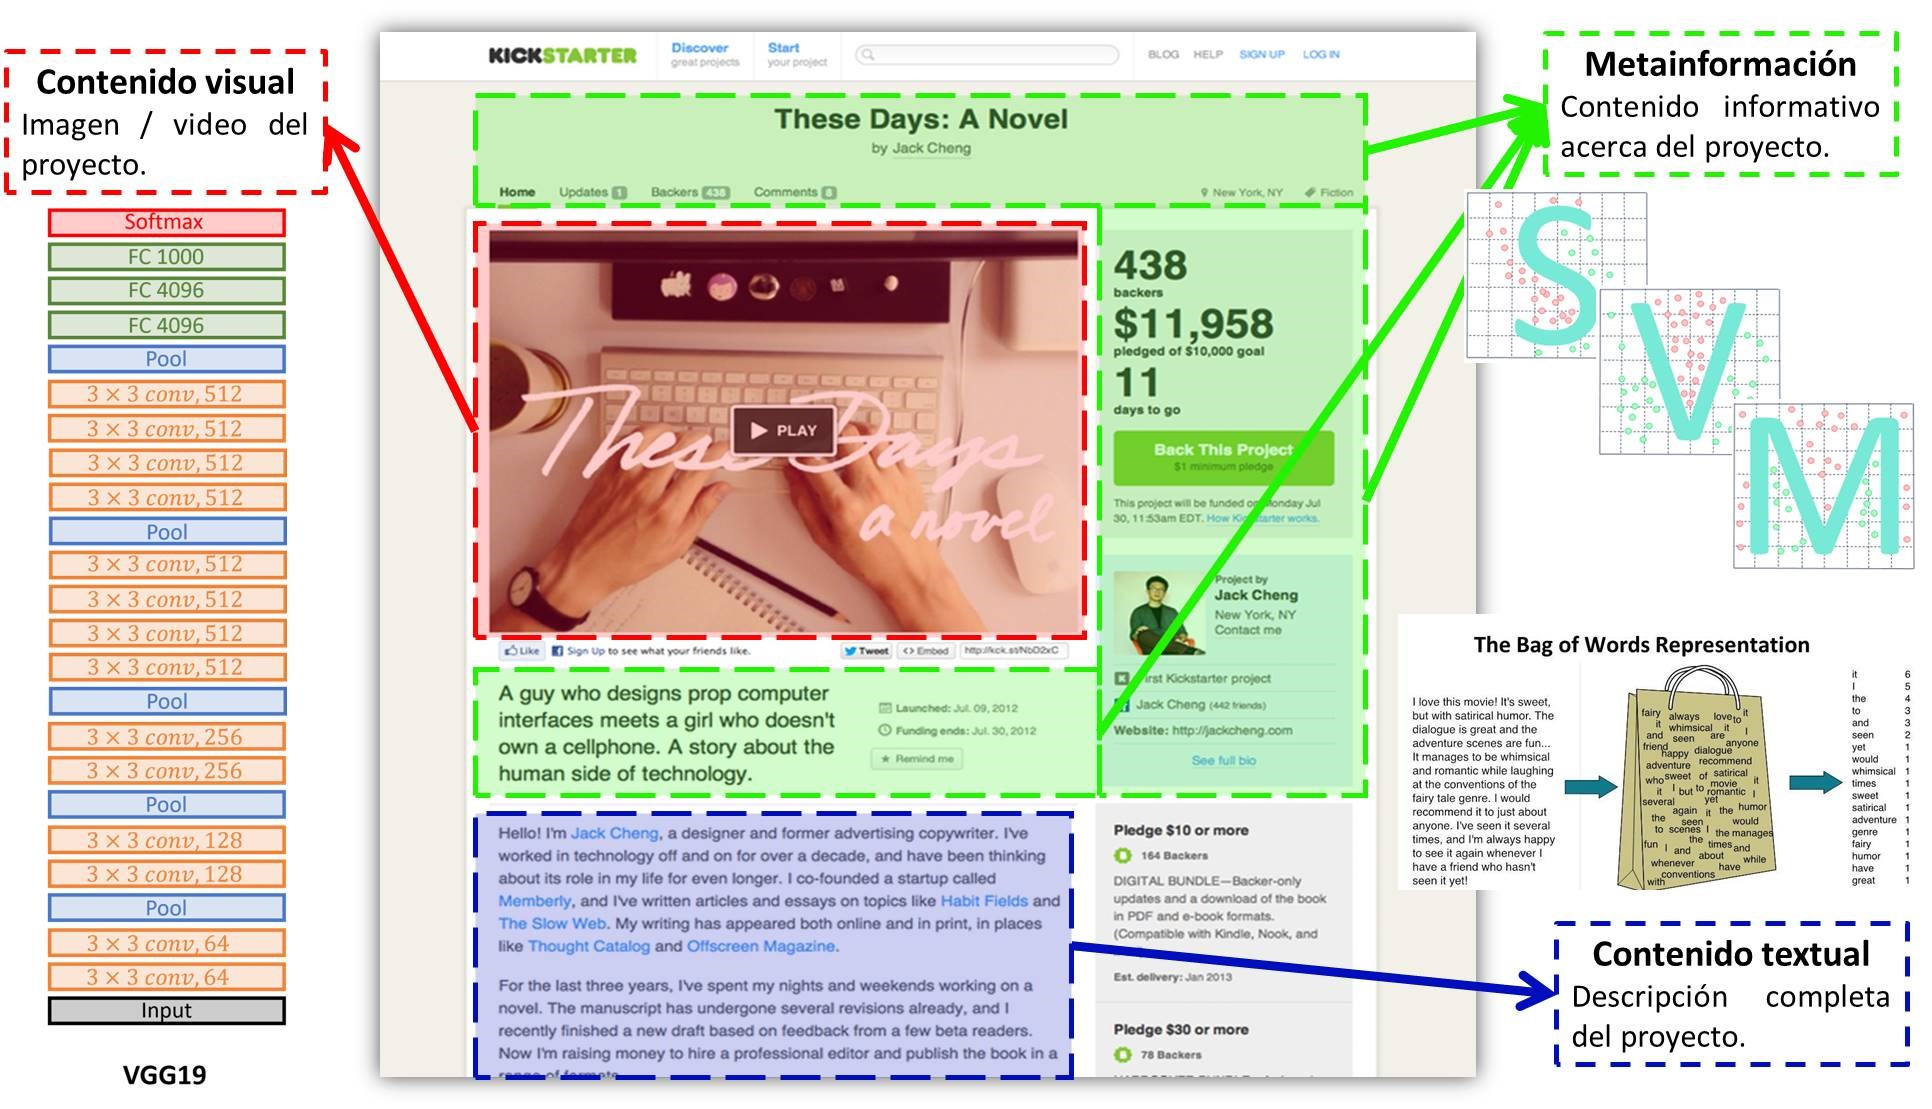
\includegraphics[width=1\textwidth]{3/figures/prototipo.jpg}
		\caption{Marco de trabajo del prototipo final. Fuente: Elaboración propia}
		\label{3:fig1}
	\end{center}
\end{figure}

\section{Población y muestra}

\subsection{Población}
La población que será considerada para el presente trabajo será de 27,251 proyectos en Kickstarter de la categoría tecnología de todas las subcategorías entre los periodos 2009-2019, en su mayoría del territorio de los Estados Unidos de América.

\subsection{Muestra}
Se distribuyeron los subconjuntos de entrenamiento y prueba en proporciones de 80\% (21,710 registros) y 20\% (5,541 registros) respectivamente (\citeauthor{pr_yuan2016textanalytics}, séptimo antecedente; \citeauthor{pr_yu2018deeplearning}, undécimo antecedente; \citeauthor{pr_chen2019keywords_crowdfunding}, decimoquinto antecedente; \citeauthor{pr_mitra2014phrases}, segundo antecedente; \citeauthor{pr_sawhney2016usingLT}, octavo antecedente).

\subsection{Unidad de análisis}
La unidad de análisis para el presente trabajo será un proyecto en Kickstarter de la categoría tecnología de cualquier subcategoría entre los periodos 2009-2019 dentro del territorio de los Estados Unidos de América.

\section{Operacionalización de Variables}
En la Tabla \ref{3:table1} se presentan las variables usadas para el conjunto de datos final basado en contenido textual y metainformación. Estas fueron seleccionadas de acuerdo al Benchmarking aplicado a los 17 antecedentes en el Capítulo II.

\begin{table}[h!]
	\centering
	\small
	\begin{tabular}{ |m{3cm}|m{10cm}|m{2cm}|  }
		\hline
		\rowcolor{bluejean}
		\Centering \color{white}{Variable}& \Centering \color{white}{Detalle}& \Centering \color{white}{Tipo de dato}\\
		\hline
		\rowcolor{turq}
		\multicolumn{3}{c}{Variables independientes} \\
		\hline
		\textbf{goal} &	Monto de la meta de financiamiento del proyecto. &	float64 \\
		\hline
		\textbf{completeness} & Porcentaje de financiamiento o completitud. & float64 \\
		\hline
		\textbf{duration} &	Duración de la campaña (en días). &	int64 \\
		\hline
		\textbf{pledges\_num} &	Cantidad de montos disponibles para contribuir. &	int64 \\
		\hline
		\textbf{pledged} &	Monto contribuído en la campaña. &	float64 \\
		\hline
		\textbf{pledges\_median} &	Mediana de montos disponibles para contribuir. &	float64 \\
		\hline
		\textbf{description} &	Descripción del proyecto. &	object \\
		\hline
		\textbf{comments} & Comentarios de patrocinadores sobre el proyecto. & object \\
		\hline
		\rowcolor{turq}
		\multicolumn{3}{c}{Variable dependiente} \\
		\hline
		\textbf{state} & Estado de financiamiento del proyecto. & object \\
		\hline
	\end{tabular}
	\caption{Diccionario de datos del conjunto final entrenado. Fuente: Elaboración propia.}
	\label{3:table1}
\end{table}

Los autores citados por cada variable utilizada se mencionan a continuación:
\begin{itemize}
	\item \textbf{goal}: \citeauthor{pr_chen2013kickpredict} (primer antecedente), \citeauthor{pr_mitra2014phrases} (segundo antecedente), \citeauthor{pr_zhou2015projectdesc} (tercer antecedente), \citeauthor{pr_chen2015predcrowd} (cuarto antecedente), \citeauthor{pr_li2016predcrowd} (sexto antecedente), \citeauthor{pr_yuan2016textanalytics} (séptimo antecedente), \citeauthor{pr_sawhney2016usingLT} (octavo antecedente), \citeauthor{pr_kaur2017socmedcrowd} (noveno antecedente), \citeauthor{pr_kamath2018suplearn} (décimo antecedente), \citeauthor{pr_yu2018deeplearning} (undécimo antecedente), \citeauthor{pr_jin2019dayssuccess} (decimotercer antecedente), \citeauthor{pr_cheng2019deeplearning} (decimocuarto antecedente).
	\item \textbf{completeness}: \citeauthor{pr_chen2015predcrowd} (cuarto antecedente).
	\item \textbf{duration}: \citeauthor{pr_mitra2014phrases} (segundo antecedente), \citeauthor{pr_zhou2015projectdesc} (tercer antecedente), \citeauthor{pr_li2016predcrowd} (sexto antecedente), \citeauthor{pr_sawhney2016usingLT} (octavo antecedente), \citeauthor{pr_kaur2017socmedcrowd} (noveno antecedente), \citeauthor{pr_kamath2018suplearn} (décimo antecedente), \citeauthor{pr_yu2018deeplearning} (undécimo antecedente), \citeauthor{pr_jin2019dayssuccess} (decimotercer antecedente).
	\item \textbf{pledges\_num}: \citeauthor{pr_chen2013kickpredict} (primer antecedente), \citeauthor{pr_mitra2014phrases} (segundo antecedente), \citeauthor{pr_chen2015predcrowd} (cuarto antecedente), \citeauthor{pr_yuan2016textanalytics} (séptimo antecedente), \citeauthor{pr_jin2019dayssuccess} (decimotercer antecedente).
	\item \textbf{pledged}: \citeauthor{pr_chen2013kickpredict} (primer antecedente), \citeauthor{pr_li2016predcrowd} (sexto antecedente), \citeauthor{pr_kamath2018suplearn} (décimo antecedente).
	\item \textbf{pledges\_median}: \citeauthor{pr_chen2015predcrowd} (cuarto antecedente)*, \citeauthor{pr_jin2019dayssuccess} (decimotercer antecedente)*.
	\item \textbf{description}: \citeauthor{pr_mitra2014phrases} (segundo antecedente), \citeauthor{pr_zhou2015projectdesc} (tercer antecedente), \citeauthor{pr_yuan2016textanalytics} (séptimo antecedente), \citeauthor{pr_sawhney2016usingLT} (octavo antecedente), \citeauthor{pr_kamath2018suplearn} (décimo antecedente), \citeauthor{pr_lee2018contentDL} (duodécimo antecedente), \citeauthor{pr_jin2019dayssuccess} (decimotercer antecedente), \citeauthor{pr_cheng2019deeplearning} (decimocuarto antecedente), \citeauthor{pr_chen2019keywords_crowdfunding} (decimoquinto antecedente), \citeauthor{pr_chaichi2019nlp_3dprinting} (decimosexto antecedente).
	\item \textbf{comments}: \citeauthor{pr_li2016predcrowd} (sexto antecedente), \citeauthor{pr_kaur2017socmedcrowd} (noveno antecedente), \citeauthor{pr_lee2018contentDL} (duodécimo antecedente), \citeauthor{pr_jin2019dayssuccess} (decimotercer antecedente).
\end{itemize}

Si bien en los respectivos antecedentes marcados en (*) figuran el promedio de los montos disponibles para patrocinar, se usó la mediana en vez de la media ya que presentó mejor performance en los experimentos.

\section{Instrumentos de medida}
Los instrumentos de medida que servirán para determinar la performance del o los modelos construidos en el experimento serán algunas de las métricas de clasificación de Machine Learning descritas en los papers tomados como antecedentes en el Capítulo II del presente trabajo y seleccionadas mediante Benchmarking considerando como criterio la similitud del problema y propuestas de solución más aproximadas. Antes de proceder a explicar detalladamente cada una de ellas, es necesario conocer los conceptos de la Matriz de confusión, así como sus elementos que la componen.

\begin{itemize}
	\item \textbf{Matriz de confusión}: Es una tabla de NxN que resume el nivel de éxito de las predicciones de un modelo de clasificación; es decir, la correlación que existe entre la etiqueta y la clasificación del modelo. Un eje de una matriz de confusión es la etiqueta que el modelo predijo; el otro es la etiqueta real. N representa el número de clases. Es un problema de clasificación binaria, N=2 \parencite{gl_kohavi1998ml_glossary}. Su principal objetivo es describir el rendimiento de un modelo supervisado de Machine Learning en los datos de prueba, donde se desconocen los verdaderos valores. Se le llama “matriz de confusión” porque hace que sea fácil detectar dónde el sistema está confundiendo dos clases \parencite{gl_bigdata2019metricas}. Se representa de la siguiente manera:
\end{itemize}

De la anterior tabla, existen 4 elementos clave:
\begin{itemize}
	\item \textbf{Verdadero positivo} (TP o \textit{True Positive}): Es el ejemplo en el que el modelo predijo de manera correcta la clase positiva. Por ejemplo, el modelo infirió correctamente que un paciente con determinadas características descritas en las variables sufre de cáncer \parencite{gl_google2018machinelearning}.
	\item \textbf{Verdadero negativo} (TN o \textit{True Negative}): Es el ejemplo en el que el modelo predijo de manera correcta la clase negativa. Por ejemplo, el modelo infirió correctamente que una determinada especie animal de acuerdo a sus características no era un mamífero \parencite{gl_google2018machinelearning}.
	\item \textbf{Falso positivo} (FP, \textit{False Positive} o Error del Tipo I): Es el ejemplo en el que el modelo predijo de manera incorrecta la clase positiva. Por ejemplo, el modelo infirió que un paciente varón presentaba embarazo (clase positiva) cuando en realidad no era así \parencite{gl_google2018machinelearning}.
	\item \textbf{Falso negativo} (FN, \textit{False Negative} o Error del Tipo II): Es el ejemplo en el que el modelo predijo de manera incorrecta la clase negativa. Por ejemplo, el modelo infirió que un mensaje de correo electrónico en particular no era spam (clase negativa), pero ese mensaje en realidad sí era spam \parencite{gl_google2018machinelearning}. 
\end{itemize}

Explicado los conceptos anteriores, se derivan las siguientes métricas de clasificación usadas comúnmente, de las cuales serán usadas solo las 3 primeras tomando como referencia los papers de los antecentes:
\begin{itemize}
	\item \textbf{Exactitud} (\textit{accuracy}): Representa la fracción de predicciones que se realizaron correctamente sobre el total de ejemplos en un modelo de clasificación. Se determina mediante la siguiente fórmula \parencite{gl_kohavi1998ml_glossary}:
	
	\begin{equcaption}[!ht]
		\begin{equation*}	
		\phantomsection
		Exactitud=\frac{V.P.+V.N.}{V.P.+V.N.+F.P.+F.N.}
		\end{equation*}
		\caption[Fórmula para calcular la exactitud. Fuente: \cite{gl_kohavi1998ml_glossary}]{Fórmula para calcular la exactitud. Fuente: \cite{gl_kohavi1998ml_glossary}}
		\label{eq:accuracy}
	\end{equcaption}
	
	Esta métrica responde a la pregunta ¿Cuál es la proporción de predicciones que se realizaron correctamente? \parencite{gl_izco2018bdc}
	
	\item \textbf{Precisión} (\textit{precision}): Representa el número de elementos identificados correctamente como positivo de un total de elementos identificados como positivos \parencite{gl_bigdata2019metricas}. Se calcula mediante la siguiente fórmula:
	
	\begin{equcaption}[!ht]
		\begin{equation*}	
		\phantomsection
		Precisi\acute{o}n=\frac{V.P.}{V.P.+F.P.}
		\end{equation*}
		\caption[Fórmula para calcular la precisión. Fuente: \cite{gl_kohavi1998ml_glossary}]{Fórmula para calcular la precisión. Fuente: \cite{gl_kohavi1998ml_glossary}}
		\label{eq:precision}
	\end{equcaption}
	
	Esta métrica responde a la pregunta ¿Qué proporción de predicciones positivas es correcta? \parencite{gl_izco2018bdc}
	
	\item \textbf{Área bajo la curva ROC} (\textit{AUC}): Considera todos los umbrales de clasificación posibles. Representa la probabilidad de que un clasificador tenga más seguridad de que un ejemplo resulte ser un verdadero positivo con respecto a que sea un falso positivo \parencite{gl_google2018machinelearning}. Para entender el concepto del área, se necesita entender qué es la curva ROC y para qué sirve en primer lugar.
	
	La curva ROC permite cuantificar la performance de distinción entre dos cosas del modelo como, por ejemplo, si un paciente tiene cáncer o no.
	
	Siguiendo el anterior ejemplo, se tiene un modelo que predice si un paciente sufre de cáncer o no, cuyo resultado es el siguiente (Figura \ref{3:fig2})
	
	\begin{figure}[htbp]
		\begin{center}
			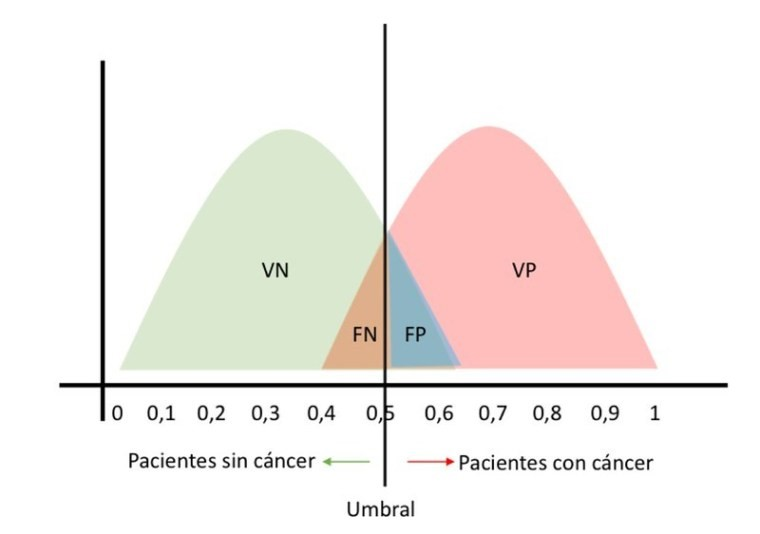
\includegraphics[width=0.7\textwidth]{3/figures/auc_example.jpg}
			\caption{Descripción de resultados de modelo descriptivo de ejemplo. Fuente: \parencite{gl_gonzalez2019auc}}
			\label{3:fig2}
		\end{center}
	\end{figure}
	
	En esta imagen, se puede observar que el área de borde verde (que contiene a los Falsos Positivos y el total de Negativos) representa a todos los pacientes que no tienen cáncer, mientras que el área de borde rojo (que contiene a los Falsos Negativos y el total de Positivos) representa a todos los pacientes que sí tienen cáncer. El umbral, que está establecido con valor 0.5, representa el punto de corte en el que el modelo clasificará a todos los pacientes por encima de ese valor como positivos, es decir, que sí tienen cáncer; mientras que aquellos por debajo del valor del umbral serán clasificados como negativos, es decir, que no tienen cáncer.
	
	Cuando el umbral se desplaza hacia la izquierda, es decir, cuando la sensibilidad aumenta, la especificidad disminuirá. Por el contrario, cuando el umbral se desplaza hacia la derecha, la sensibilidad disminuirá y la especificidad aumentará. Se concluye entonces que existe una relación inversa entre la sensibilidad y la especificidad. En la curva ROC se representa la sensitividad (1-especificidad) \parencite{gl_gonzalez2019auc}.
	
	Ahora bien, el área que se grafica bajo esta curva explicará qué tan bien funciona el modelo. Este tendrá un mejor desempeño si la curva se aleja de la diagonal principal como se observa en la Figura \ref{3:fig3}.
	
	\begin{figure}[htbp]
		\begin{center}
			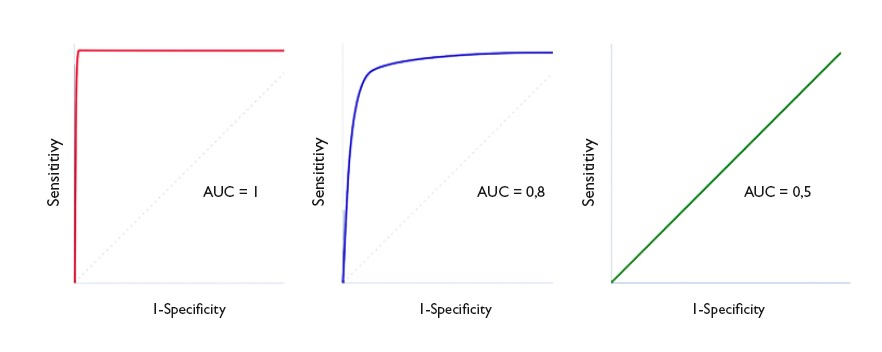
\includegraphics[width=0.9\textwidth]{3/figures/auc_curves.jpg}
			\caption{Comparación de tres resultados de la curva AUC en el modelo. Fuente: \parencite{pr_molina2017pediatria_curvaroc}}
			\label{3:fig3}
		\end{center}
	\end{figure}
	
	Una interpretación básica del área bajo la curva ROC respecto del poder discriminante del modelo se muestra a continuación \parencite{bk_britos2006datamining}:
	\begin{itemize}
		\item Si el área bajo la curva ROC = 0.5, entonces el poder discriminante del modelo es nulo.
		\item Si el área bajo la curva 0.5 $<$ ROC $<$ 0.7, entonces el poder discriminante del modelo no es aceptable.
		\item Si el área bajo la curva 0.7 $\leq$ ROC $<$ 0.8, entonces el poder discriminante del modelo es aceptable.
		\item Si el área bajo la curva 0.8 $\leq$ ROC $<$ 0.9, entonces el poder discriminante del modelo es excelente.
		\item Si el área bajo la curva ROC $\geq$ 0.9, entonces el poder discriminante del modelo es excepcionalmente bueno.
	\end{itemize}
	\item \textbf{Sensibilidad} (\textit{recall}, \textit{sensitivity} o \textit{True Positive Rate}): Representa el número de elementos correctamente identificados como positivos del total de positivos verdaderos \parencite{gl_bigdata2019metricas}. Se calcula mediante la siguiente fórmula:
	
	\begin{equcaption}[!ht]
		\begin{equation*}	
		\phantomsection
		Sensibilidad=\frac{V.P.}{V.P.+F.N.}
		\end{equation*}
		\caption[Fórmula para calcular la sensibilidad. Fuente: \cite{gl_kohavi1998ml_glossary}]{Fórmula para calcular la sensibilidad. Fuente: \cite{gl_kohavi1998ml_glossary}}
		\label{eq:recall}
	\end{equcaption}
	
	\item \textbf{Puntaje F1} (\textit{F1-Score}): Representa la media armónica de la precisión y la sensibilidad. Normalmente, se usa cuando uno difiere mucho del otro y no es posible realizar una conclusión determinante ya que solo es posible predecir bien una clase \parencite{gl_bigdata2019metricas}. Se calcula mediante la siguiente fórmula:
	
	\begin{equcaption}[!ht]
		\begin{equation*}	
		\phantomsection
		Puntaje F1=\frac{2*Precisi\acute{o}n*Sensibilidad}{Precisi\acute{o}n+Sensibilidad}
		\end{equation*}
		\caption[Fórmula para calcular el puntaje F1. Fuente: \cite{gl_kohavi1998ml_glossary}]{Fórmula para calcular el puntaje F1. Fuente: \cite{gl_kohavi1998ml_glossary}}
		\label{eq:f1-score}
	\end{equcaption}
	
\end{itemize}

\section{Técnicas de recolección de datos}
Los conjuntos de datos recolectados para la investigación se componen de mezcla de observaciones cuantitativas (variables numéricas basadas en características del proyecto como la meta de financiamiento, montos prometidos, duración de la campaña y otros indicadores financieros) y cualitativas (descripción y comentarios del proyecto). Para obtener los 3 principales datasets, se siguió el flujo de la Figura \ref{3:fig4}. La base de datos de la metainformación, que comprende las variables cuantitativas y propaganda del proyecto, fue consolidada luego de descargar un histórico público de 10 años de la página web “Web Robots”, fundada por los ex corporativos de TI Tomás Vitulskis y Paulius Jonaitis, y posteriormente pre-procesarla. Mientras que por el lado de la descripción y comentarios de cada proyecto, se usaron técnicas y herramientas de \textit{web scraping} a partir de los URLs. El detalle de cada paso del proceso se explica en la sección de Construcción de los conjuntos finales de datos del Capítulo IV.

\begin{figure}[h]
	\begin{center}
		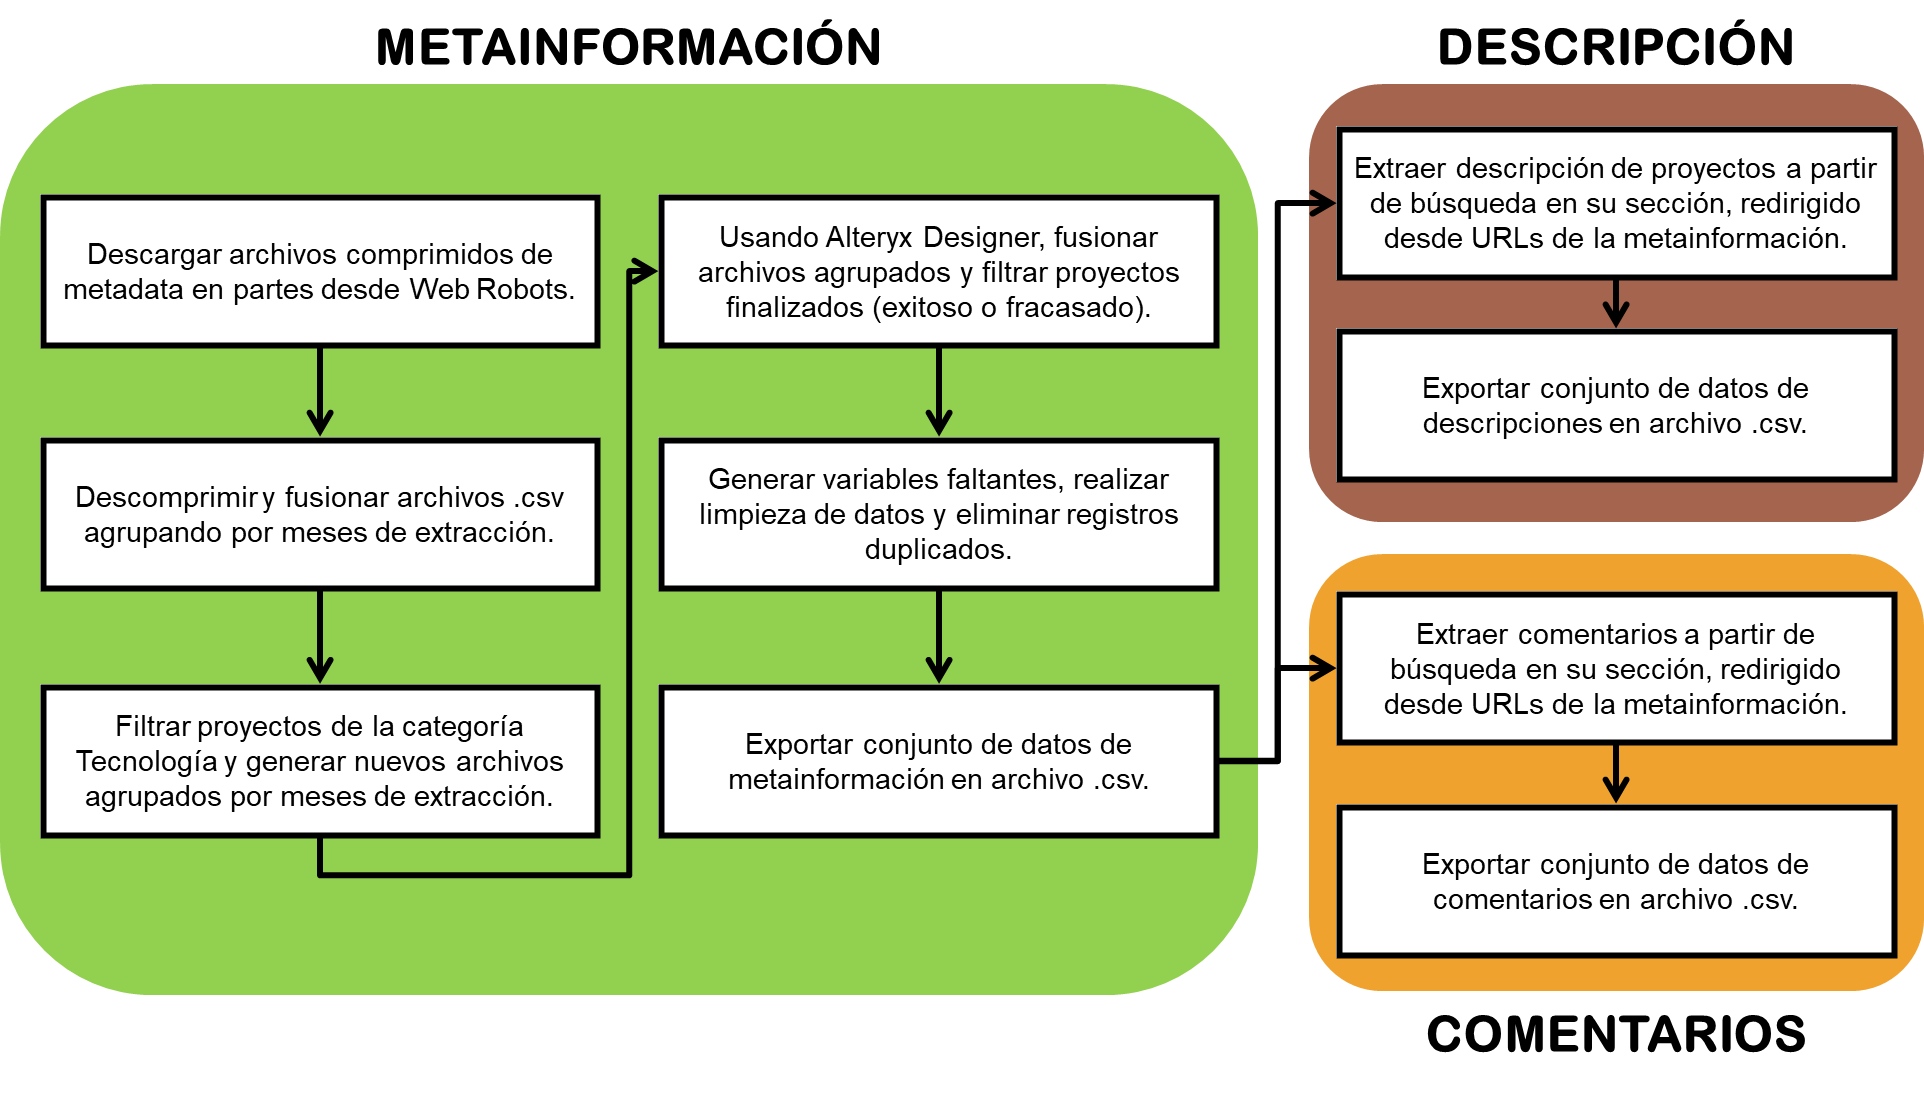
\includegraphics[width=0.95\textwidth]{3/figures/data_recolection_flux.png}
		\caption{Flujograma de la recolección de conjuntos finales de datos. Fuente: Elaboración propia.}
		\label{3:fig4}
	\end{center}
\end{figure}

Asimismo, para encontrar algunos de los papers con la información requerida más cercana, se utilizaron keywords o palabras clave como \textit{crowdfunding}, \textit{Machine Learning}, \textit{Deep Learning}, \textit{prediction}, \textit{Kickstarter}, \textit{accuracy} y \textit{projects}.

\section{Técnicas para el procesamiento y análisis de la información}



\section{Cronograma de actividades y presupuesto}
Se elaboró un cronograma de actividades de toda la investigación, mostrada en la Figura \ref{3:fig5}, contemplando desde el inicio de la misma, desarrollo, evaluación de resultados y sustentación en el mes de diciembre.
\begin{figure}[h]
	\begin{center}
		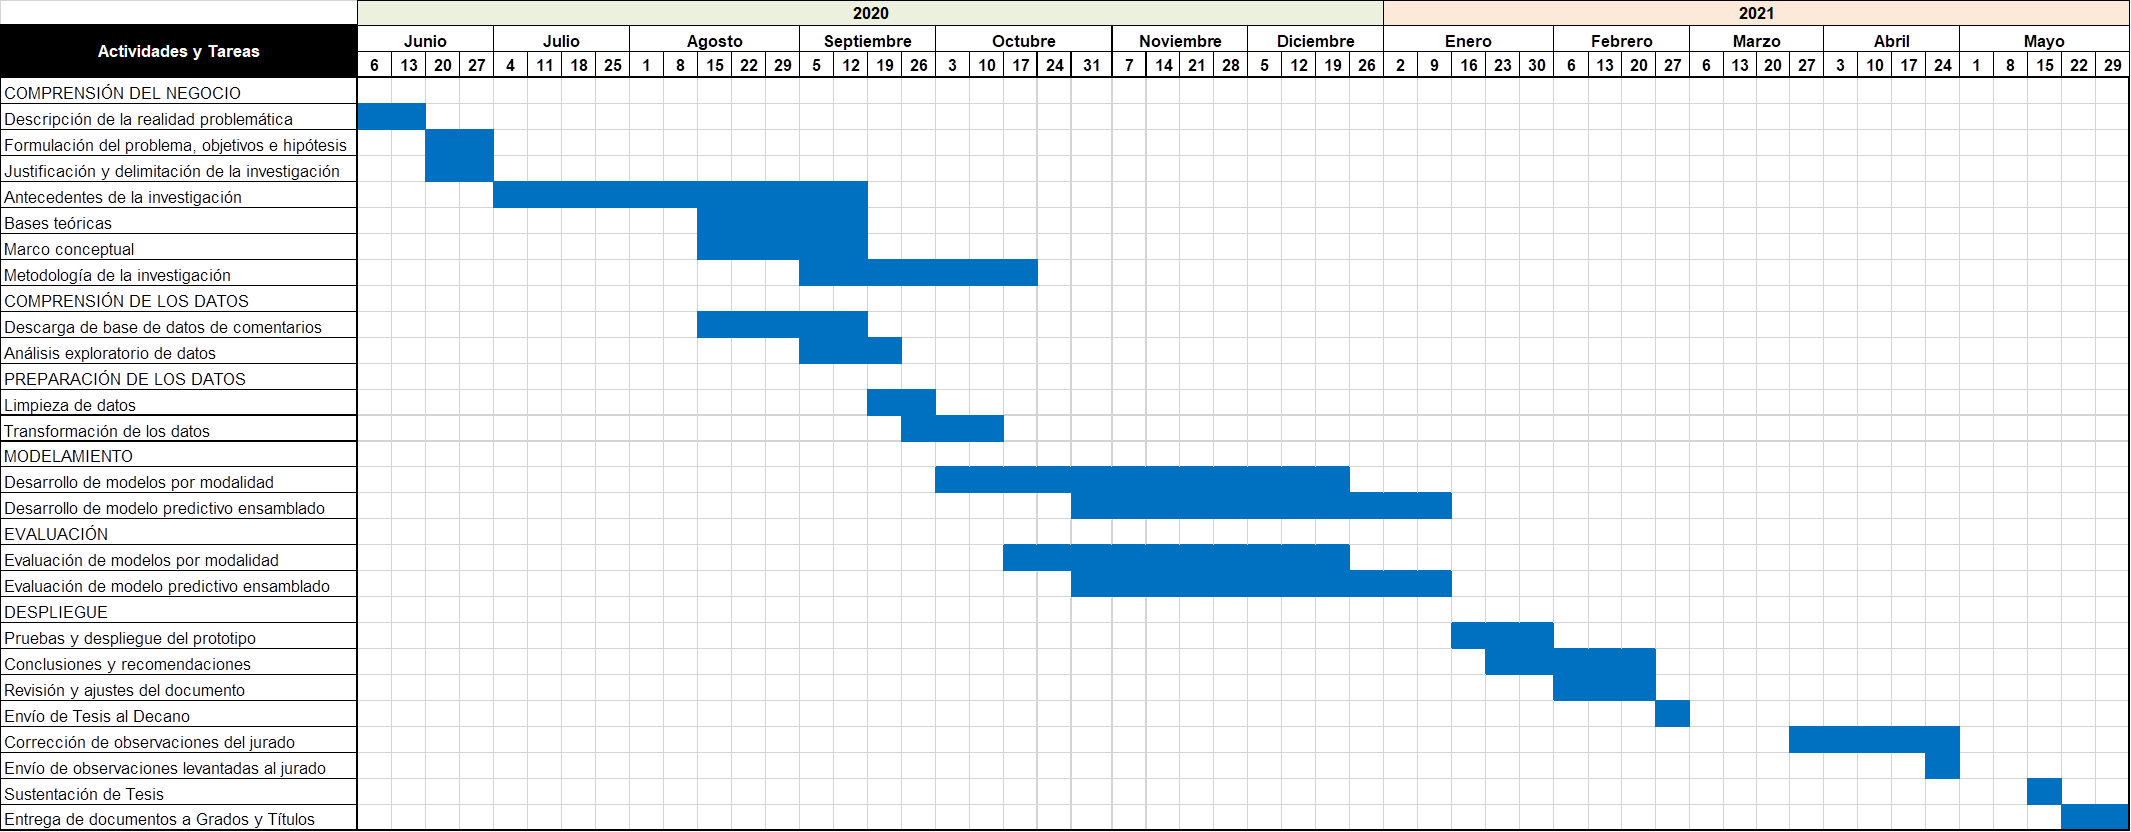
\includegraphics[width=1.1\textwidth]{3/figures/cronograma.png}
		\caption{Cronograma de actividades de la investigación. Fuente: Elaboración propia}
		\label{3:fig5}
	\end{center}
\end{figure}